\documentclass[10pt, oneside,spanish]{article}   	% use "amsart" instead of "article" for AMSLaTeX format
\usepackage{geometry}                		% See geometry.pdf to learn the layout options. There are lots.
\geometry{a4paper}                   		% ... or a4paper or a5paper or ... 
\usepackage[spanish, es-noindentfirst]{babel}
\selectlanguage{spanish}
\usepackage[utf8]{inputenc}
%\geometry{landscape}                		% Activate for rotated page geometry
%\usepackage[parfill]{parskip}    		% Activate to begin paragraphs with an empty line rather than an indent
\usepackage{graphicx}				% Use pdf, png, jpg, or eps§ with pdflatex; use eps in DVI mode
								% TeX will automatically convert eps --> pdf in pdflatex		
\usepackage{amssymb}
\usepackage{authblk}
%SetFonts

%SetFonts

\title{Reporte de Laboratorio Nro. escriba el número}
\author[IDEstudiante]{Nombre Apellido Estudiante}
\affil[ ]{Universidad de las Fuerzas Armadas}
\affil[ ]{email@dominio.ec}
\affil[ ]{}
\affil[ ]{Tema: Tema de Laboratorio}
\renewcommand\Authands{, }
\date{}							% Activate to display a given date or no date

\begin{document}
\maketitle

\begin{abstract}
Escriba aquí un breve resumen del laboratorio, el cual se utiliza para ayudar al lector a determinar rápidamente el propósito de su reporte. Escribir únicamente un párrafo, el cuál puede tener al menos 100 palabras, pero no más de 200.
\end{abstract}

\section{Introducción}
En esta sección brindará información general sobre el laboratorio o taller. Aquí también es donde se explica los objetivos del experimento~\cite{fest1959}. Esta sección debe tener al menos 3 párrafos, los cuales deben estar formados por al menos 4 oraciones.

\section {Método}
Describe lo que hiciste (no los nombres de archivos y directorios, por supuesto, sino todos los pasos importantes que te llevan a los resultados). ¿Por qué hiciste esto? ¿Tuviste que tomar algunas decisiones en el camino? Explícalas. ¿No funcionó bien la primera vez y tenías que mejorar algo? Escribe sobre eso.

Incluya diagramas/fotos de la configuración experimental (vea la Figura~\ref{fig1}) o capturas de pantalla que destaquen los pasos importantes del proceso.

\begin{figure*}[!ht] 
        \centering 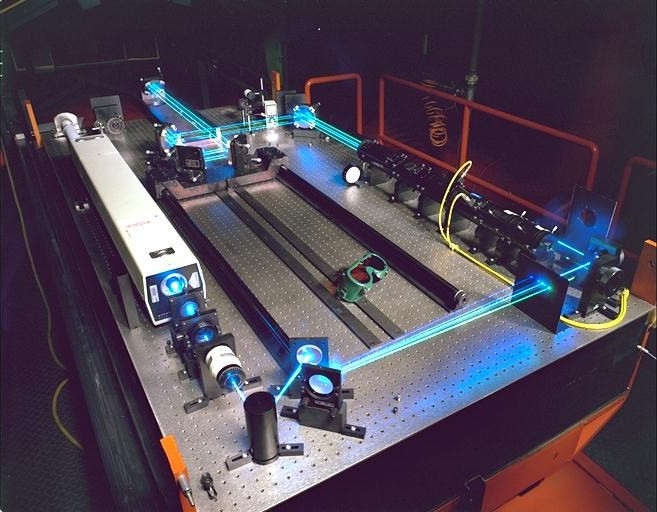
\includegraphics[width=0.5\columnwidth]{Laser.jpg}
        \caption{\label{fig1}Every figure MUST have a caption~\cite{fest1959}.
        }
\end{figure*}

\section{Results and Analysis}
En esta sección, deberá mostrar sus resultados. Utilice tablas y cifras (se pueden incluir tablas largas en un apéndice). La tabla~\ref{table1} es un ejemplo.

\begin{table*}[ht]
\begin{center}
\caption{Cada tabla necesita una leyenda.}
\label{table1} 
\begin{tabular}{cc} 
\hline
\multicolumn{1}{c}{distance (m)} & \multicolumn{1}{c}{V (km s$^-1$)} \\
\hline
0.0044151 &   0.0030871 \\
0.0021633 &   0.0021343 \\
0.0003600 &   0.0018642 \\
0.0023831 &   0.0013287 \\
\hline
\end{tabular}
\end{center}
\end{table*}

A continuación, explique cómo se determinan las incertidumbres para diferentes
valores medidos (de ser el caso).

Si en el proceso de análisis de datos encontró algún sistema error(s), debe explicarlos en esta sección del informe (de ser el caso). 

\section{Discusión}
Aquí resuma brevemente sus hallazgos. Además, en esta sección se constarán las preguntas existentes en la guía de laboratorio (de ser el caso). Las respuestas a las preguntas deben estar escritas en prosa, es decir evite incluir ítems.

\section{Conclusión}
Escriba la o las conclusiones del taller o laboratorio. Evite enumerar las conclusiones, escriba párrafos concisos.

\nocite{*}
\bibliographystyle{plain}
\bibliography{paper}

\end{document}  